\chapter{Introduction}


Introduction: work in progress. \\

For now the focus is on the thesis core itself. \\
Chapters do contain sub-conclusions / summaries 


\section{Background}


\section{Research gap}

\textbf{ASR systems}

blabla
\begin{figure}[h!]
	\centering
	\begin{subfigure}[b]{0.5\linewidth}
		\centering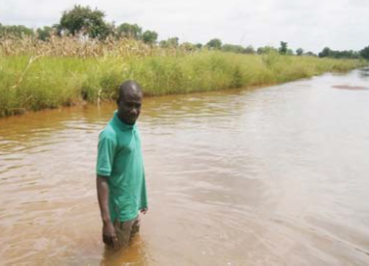
\includegraphics[width=0.8\linewidth]{Flood}
		\captionsetup{justification=centering}		
		\caption{\label{fig:Flood}}
		\end{subfigure}%\hfill
	\begin{subfigure}[b]{0.5\linewidth}
        \centering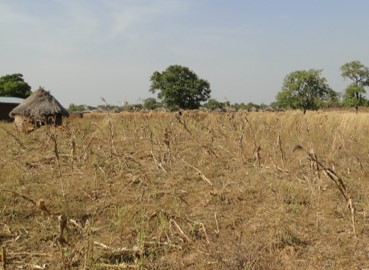
\includegraphics[width=0.8\linewidth]{Drought}
		\captionsetup{justification=centering}		
		\caption{\label{fig:Drought}}
		\end{subfigure}
		\captionsetup{justification=centering}	
	\caption[Example on (\subref{fig:Flood}) flood near Weisi, Upper West Region and (\subref{fig:Drought}) drought near Nungo, Upper East Region]{Example on (\subref{fig:Flood}) flood near Weisi, Upper West Region (source: Owusu et al., 2017) and (\subref{fig:Drought}) drought near Nungo, Upper East Region} 
	\label{fig:Flood_Drought}
\end{figure} \\

\begin{figure}[h]
 \centering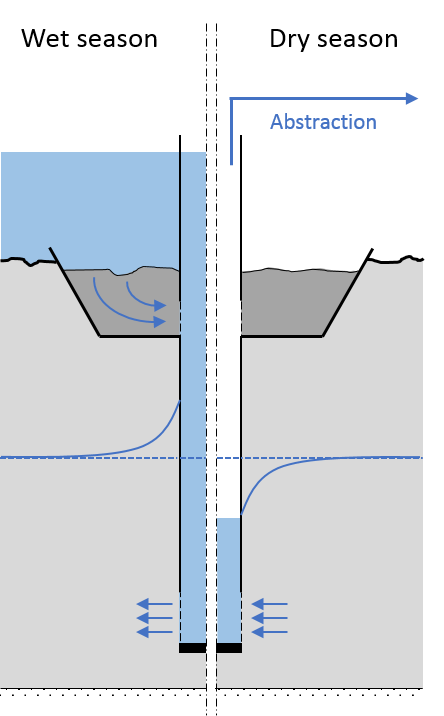
\includegraphics[width=0.4\linewidth]{Wet_Dry}
 \captionsetup{justification=centering}
 \caption{Principle Aquifer Storage \& Recovery (ASR) system}
 \label{fig:ASR}
\end{figure}

\section{Research purpose}\

\textbf{PIT \& Irrigation purpose} \\
PIT application on irrigation (single figure). and the desired upscaling of this system (multiple figure). \\

\begin{figure}[h]
 \centering
\includegraphics[width=0.8\linewidth]{Purpose}
 \captionsetup{justification=centering}
 \caption[Schematic: dry season system use]{Schematic: dry season system use \\ (visual support by Housin Aziz, Jhun Capaya and Nibras@design from Noun Project - \url{https://thenounproject.com})}
 \label{fig:Purpose}
\end{figure}

\begin{figure}[h]
 \centering
\includegraphics[width=0.8\linewidth]{Purpose_Multi}
 \captionsetup{justification=centering}
 \caption[Schematic: desired up-scaling in dry season system use]{Schematic: desired up-scaling in dry season system use \\ (visual support by Housin Aziz, Jhun Capaya and Nibras@design from Noun Project - \url{https://thenounproject.com})}
 \label{fig:Purpose_Multi}
\end{figure}

\textbf{Research question}\\

How can scaled-up Aquifer Storage and Recovery (ASR) systems be beneficial for the availability and sustainable use of groundwater in northern Ghana small-scale agriculture? \\

\section{Reader's guide}\
to answer this research question... 
